\begin{figure}[!t]
\begin{subfigure}{\linewidth}
\centering
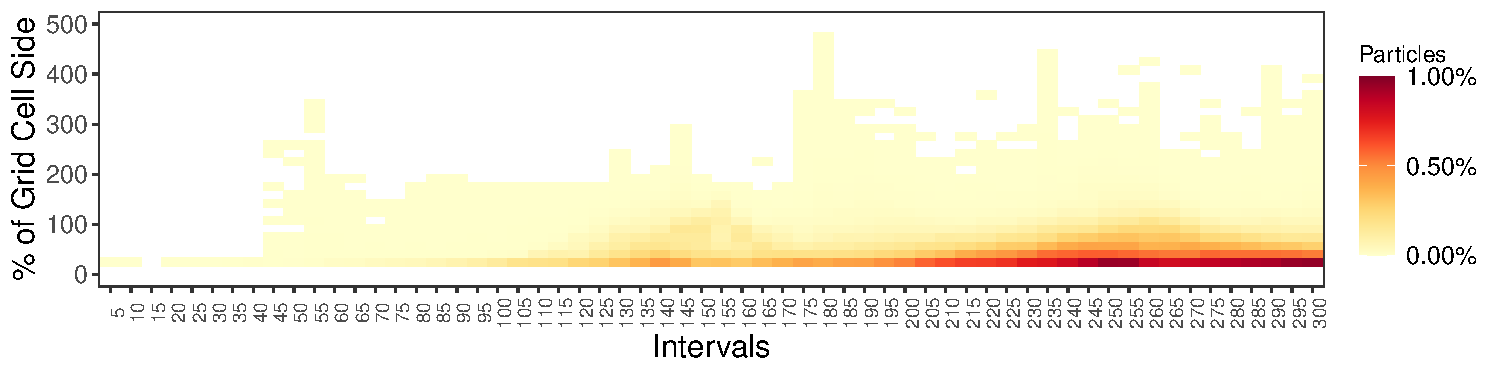
\includegraphics[width=\linewidth]{Images/Jet_Intervals_T1_Percent.pdf}
\caption{T1, 1:1}
\label{fig:jet_1}
\end{subfigure}
%\begin{subfigure}{\linewidth}
%\centering
%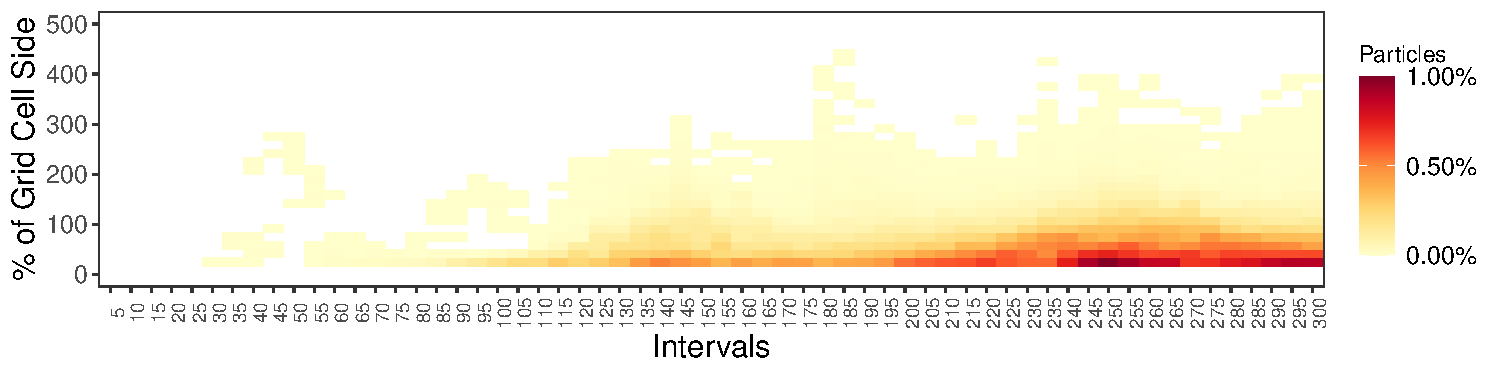
\includegraphics[width=\linewidth]{Images/Jet_Intervals_T3_Percent.pdf}
%\caption{T3, 1:8}
%\label{fig:jet_3}
%\end{subfigure}
%\begin{subfigure}{\linewidth}
%\centering
%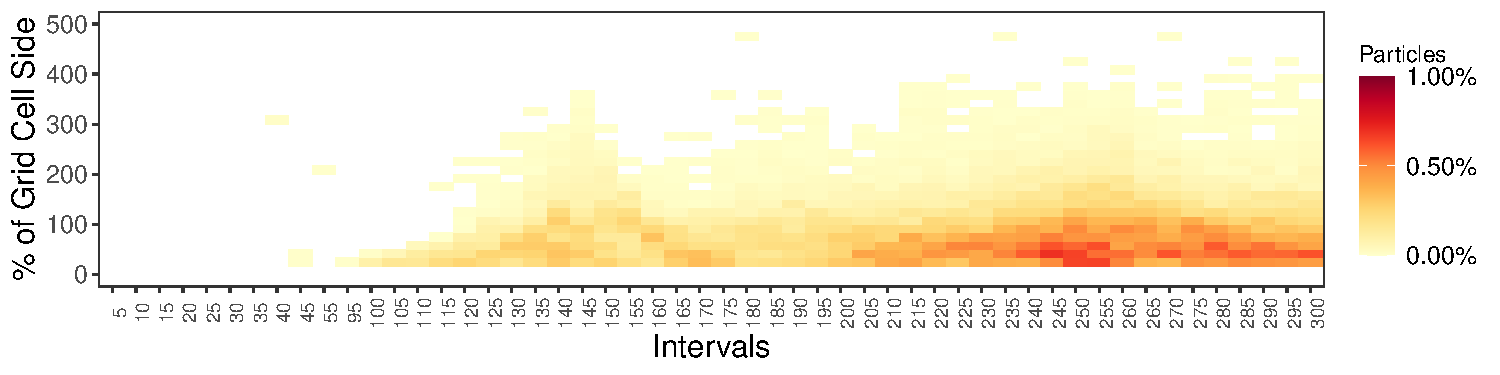
\includegraphics[width=\linewidth]{Images/Jet_Intervals_T5_Percent.pdf}
%\caption{T5, 1:27}
%\label{fig:jet_5}
%\end{subfigure}
\begin{subfigure}{\linewidth}
\centering
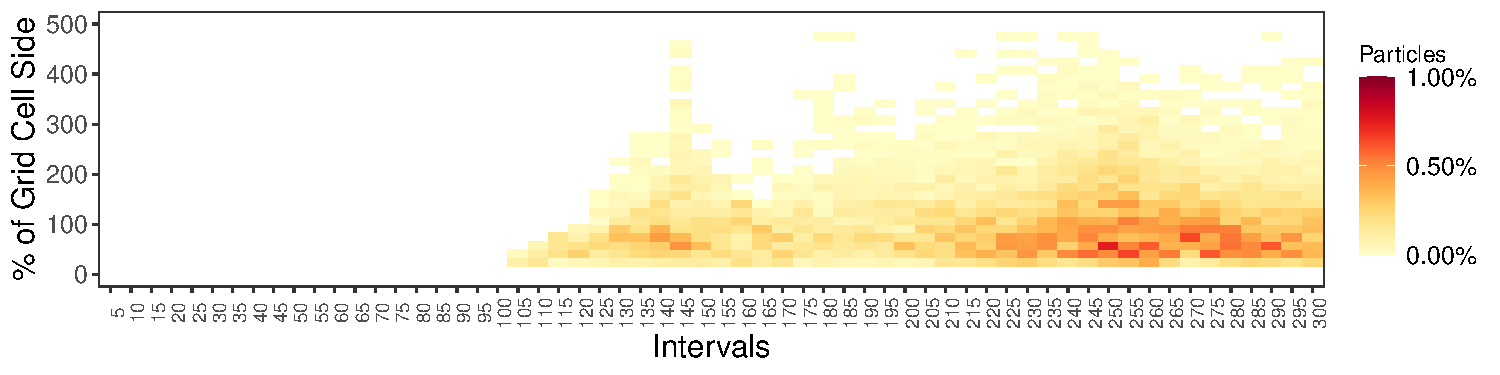
\includegraphics[width=\linewidth]{Images/Jet_Intervals_T7_Percent.pdf}
\caption{T7, 1:64}
\label{fig:jet_7}
\end{subfigure}
\caption{\fix{Heatmaps of reconstruction error for the Jet data set. These plots highlight the low tolerance for data reduction for this data set --- a high data reduction factor resulted in an increase in the percentage of particles reconstructed up to a few grid cell sides away from the ground truth.}} 
\vspace{-5mm}
\label{fig:jet_map}
\end{figure}
